\chapter{Drucken der Abschlussarbeit}
\label{cha:Drucken}


\section{PDF-Workflow}
\label{sec:pdf}

Heutzutage wird \latex\ praktisch immer so benutzt, dass damit direkt PDF-Dokumente
(ohne den früher üblichen Umweg über DVI und PostScript) erzeugt werden.
In modernen Editoren (\zB \emph{TeXstudio} oder \emph{Overleaf}) funktioniert dies
ohne weiteren Konfigurationsaufwand.


\subsection{PDF Archivformat (PDF/A)}
\label{sec:PDFA}

Viele Institutionen verlangen die Abgabe von Abschlussarbeiten im PDF/A-Format, einer
standardisierten Variante von PDF für die Langzeitarchivierung.%
\footnote{\url{https://de.wikipedia.org/wiki/PDF/A}}
Dieses Dokument wird standardmäßig im PDF/A-Format (PDF/A-2b, um genau zu sein),
aufgrund der Anweisung
%
\begin{LaTeXCode}[numbers=none]
\RequirePackage{hgbpdfa}
\end{LaTeXCode}
%
am Beginn der Datei \verb!main.tex! (wodurch \verb!hgbpdfa.sty! geladen wird).
Man beachte, dass diese Anweisung \emph{vor} der \verb!\documentclass!-Deklaration
platziert werden muss. Erforderliche Meta\-daten (\zB Autor*in und Titel) werden
automatisch aus den Dokumenteinstellungen übernommen und in das Ausgabe-PDF eingefügt.%
\footnote{Dieses Setup basiert auf neuer Funktionalität, die aktuell in den
\texttt{pdflatex}-Kern eingebaut wird und erfordert das Paket 
\texttt{pdfmanagement-testphase} in Version 0.95s (2022-09-26) oder höher.
Bei älteren Versionen wird eine Warnung ausgegeben und keine PDF/A-konforme
Ausgabe erzeugt.}


\subsection{PDF/A Problemstellen}
\label{sec:PDFA-issues}

Die Aktivierung der PDF/A-Option erzeugt eine Ausgabedatei, die \emph{vorgibt},
PDF/A-konform zu sein, was aber nicht bedeutet, dass sie es tatsächlich \emph{ist}.
Obwohl dieses Dokument ein PDF/A-konformes Dokument erzeugt, ist dies bei abgeleiteten
Dokumenten möglicherweise nicht der Fall. Es ist daher wichtig, die resultierende
PDF-Datei vor der Abgabe mit einer der unten beschriebenen Methoden zu 
\emph{validieren}. Die meisten Verletzungen des PDF/A-Standards entstehen durch 
die Einbindung anderer PDF-Dateien, insbesondere von Grafiken. Typische Probleme 
sind die Verwendung von nicht eingebetteten Schriftarten und falschen oder 
unerwünschten Farbräumen. Im aktuellen Setup wird von sRGB-Farben ausgegangen, die man
grundsätzlich auch bei der Erstellung eigener Illustrationen verwenden sollte.

Probleme mit importierten PDF-Dateien können im finalen (zusammengesetzten) Dokument
schwer zu lokalisieren sein. Wenn die problematische Datei bekannt ist und nicht 
neu generiert werden kann, lässt sie sich eventuell mit anderen Tools wie Adobe \emph{Acrobat} 
(\emph{Distiller}) oder \emph{Ghostscript}%
\footnote{\url{https://ghostscript.com/}}
reparieren.


\subsection{PDF/A Validierung}
\label{sec:PDFA-validation}

Eine einfache (und kostenlose) Methode zur Überprüfung der PDF/A-Konformität bietet
\textsf{veraPDF} in zwei Varianten:
%
\begin{itemize}
\item eine Open-Source-Validierungssoftware%
  \footnote{\url{https://verapdf.org/software} (Windows, macOS, Linux)} sowie
\item ein Online-Validierungsservice.%
  \footnote{\url{https://demo.verapdf.org}}
\end{itemize}
%
Abbildung \ref{fig:verapdf-report} zeigt ein Beispiel. Ein ähnliches Service bietet
auch \textsf{pdf-online.com},%
\footnote{\url{https://www.pdf-online.com/osa/validate.aspx}}
dessen Einstellung leider bereits angekündigt ist.
Natürlich ist die PDF/A-Validierung auch im Werkzeugsatz von Adobe \emph{Acrobat} enthalten.

\begin{figure}[htbp]
    \centering
    \fbox{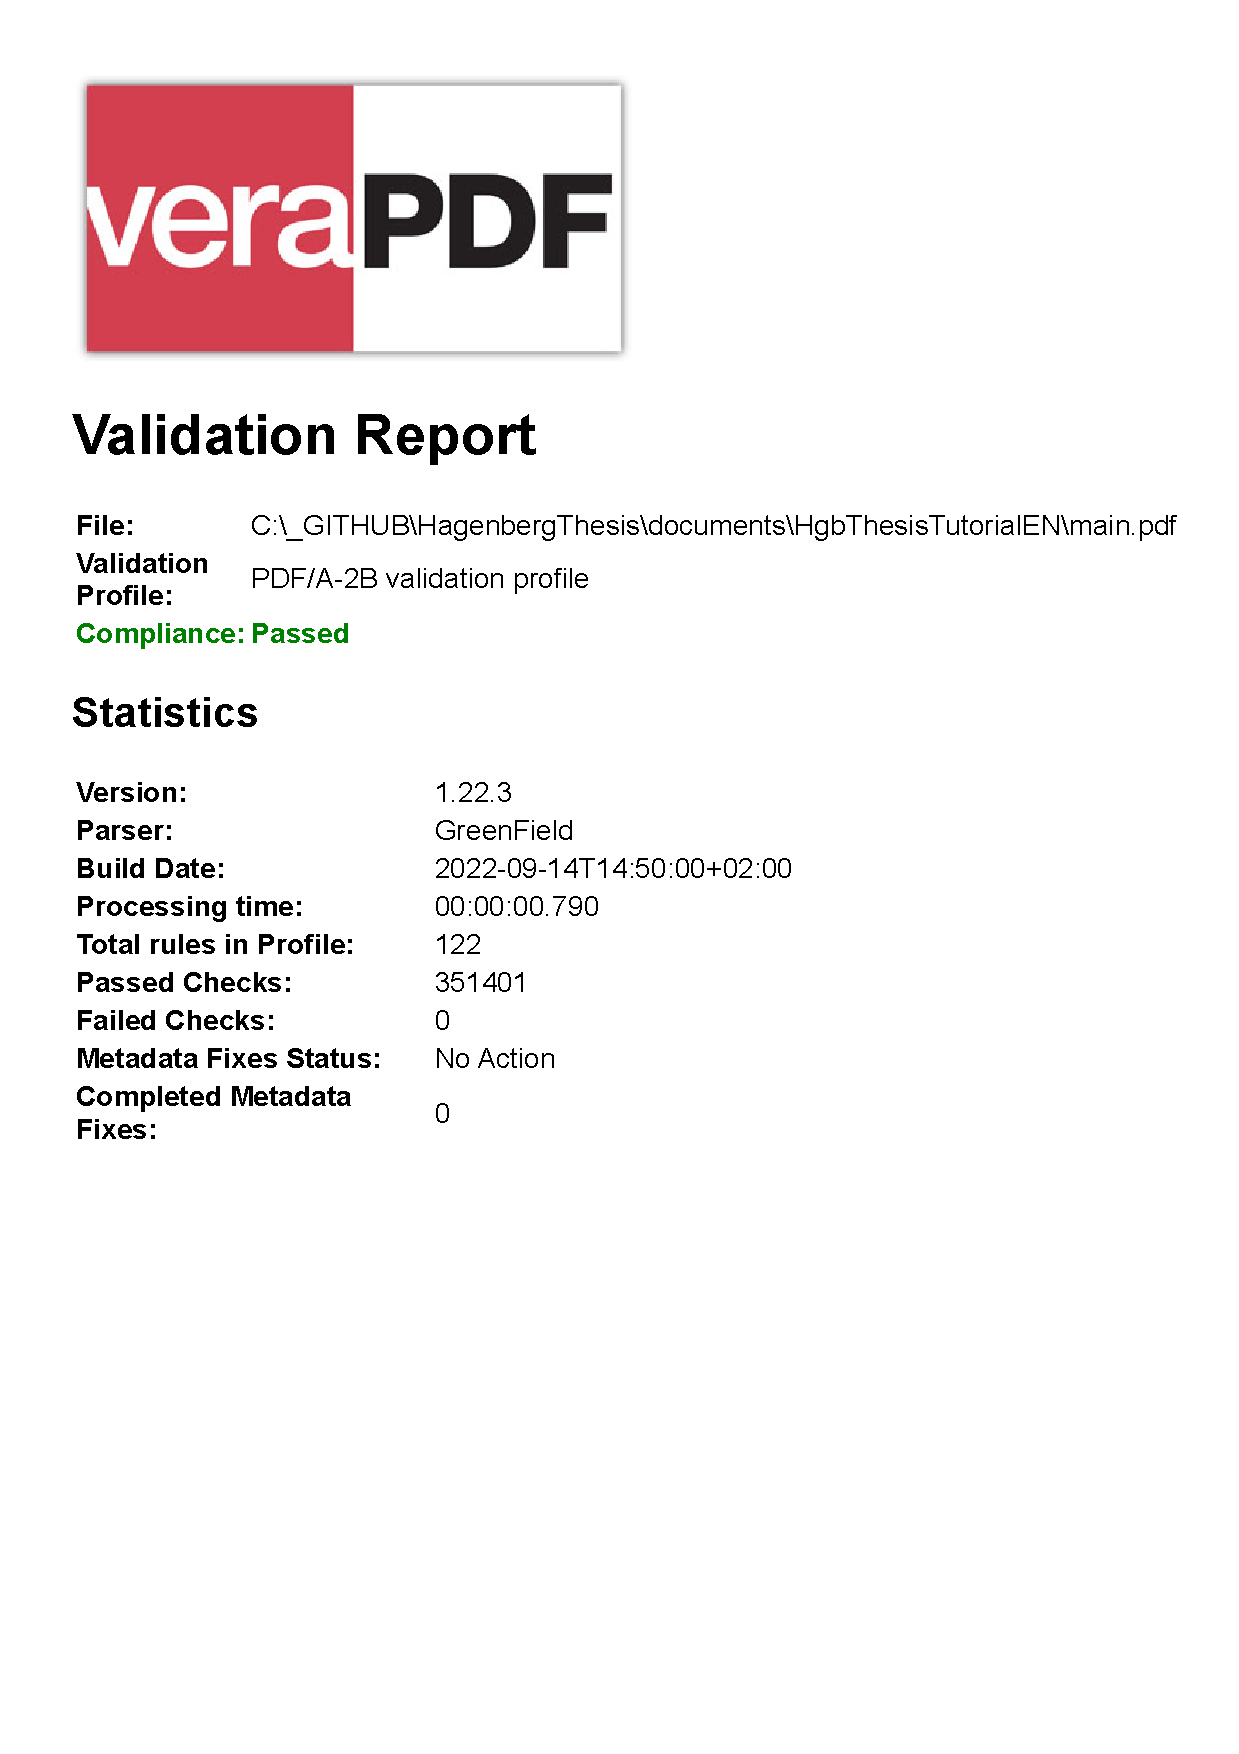
\includegraphics[width=.60\textwidth]{verapdf-report}}
    \caption{Bericht, der vom \textsf{veraPDF}-Client nach erfolgreicher Validierung 
    \emph{dieses} Dokuments erstellt wurde. Man beachte, dass der als PDF importierte Screenshot 
    selbst \emph{nicht} PDF/A-konform ist.}
    \label{fig:verapdf-report}
\end{figure}


\section{Drucken}

Vor dem Drucken der Arbeit empfiehlt es sich, einige Dinge zu beachten, um
unnötigen Aufwand (und auch Kosten) zu vermeiden.

\subsection{Digitale Abgabe oder Druck}

Viele Studiengänge verlangen mittlerweile aus Gründen der Nachhaltigkeit -- vor
allem bei Bachelorarbeiten -- keine gedruckte Abgabe mehr. Ein Upload der
PDF-Datei genügt in diesem Fall. Die Erklärung wird dann entweder digital im
Dokument signiert oder der Studiengang holt die Erklärung auf andere Art und
Weise ein. Es empfiehlt sich, die Abgabemodalitäten rechtzeitig in Erfahrung zu
bringen, um ein unnötiges Ausdrucken der Arbeit zu vermeiden.

\subsection{Drucker und Papier}

Wenn die Abschlussarbeit gedruckt wird, sollte dies in der Endfassung unbedingt
auf einem qualitativ hochwertigen \emph{Laserdrucker} geschehen; Ausdrucke mit
Tintenstrahldruckern sind \emph{nicht} ausreichend. Auch das verwendete
Papier sollte von guter Qualität (holzfrei) und üblicher Stärke (typ.\  
$80\,\mathrm{g} / \mathrm{m}^2$) sein. Falls nur einzelne \emph{farbige} Seiten 
notwendig sind, kann man diese auch einzeln auf einem Farb-Laserdrucker ausdrucken
und dem übrigen (schwarz/weiß gedruckten) Dokument beifügen.

Übrigens sollten \emph{alle} abzugebenden Exemplare \emph{gedruckt} (und
nicht kopiert) werden! Die Kosten für den Druck sind nicht höher als die für
Kopien, der Qualitätsunterschied ist jedoch -- \va\ bei Bildern und Grafiken
-- meist deutlich.

\subsection{Druckgröße}

Zunächst sollte sichergestellt werden, dass die in der fertigen PDF-Datei
eingestellte Papiergröße tatsächlich \textrm{A4} ist! Das geht \zB\ mit
\emph{Adobe Acrobat} oder \emph{SumatraPDF} über \texttt{File} $\rightarrow$
\texttt{Properties}, wo die Papiergröße des Dokuments angezeigt wird:
\begin{center}
	\textrm{Richtig:} A4 = $8{,}27 \times 11{,}69$ in \bzw\ $210 \times 297$ mm.
\end{center}
Falls das nicht übereinstimmt, ist vermutlich irgendwo im Workflow versehentlich
"Letter" als Papierformat eingestellt.


Ein häufiger und leicht zu übersehender Fehler beim Ausdrucken von
PDF-Doku\-menten wird durch die versehentliche Einstellung der Option "Fit to
page" im Druckmenü verursacht, wobei die Seiten meist zu klein ausgedruckt
werden. Überprüfen Sie daher die Größe des Ausdrucks anhand der eingestellten
Textbreite%
\footnote{\Convert[unit=mm]{\the\textwidth}	im aktuellen Dokument} % using 'lengthconvert' package
oder mithilfe der Messgrafik am Ende dieses Dokuments gezeigt.
Sicherheitshalber sollte diese Messgrafik bis zur Fertigstellung der
Arbeit beibehalten und die entsprechende Seite erst ganz am Schluss
entfernt werden. Wenn, wie häufig der Fall, einzelne Seiten getrennt in Farbe
gedruckt werden, so sollten natürlich auch diese genau auf die Einhaltung der
Druckgröße kontrolliert werden!